\section{Differential Decay Rate for \texorpdfstring{\BstoJpsiKK{}}{Bs0->JpsiKK}}
\label{sec:pheno_decay}

With four particles in the final state, the kinematics of the \BstoJpsimumuKK{} decay are described by sixteen variables. All final-state
particles are assumed to be on their mass shell, which gives four relations between the particle energies and three-momenta and only twelve
degrees of freedom remain. The final-state momenta can be expressed in terms of the four-momentum of the $\Bs$, three Euler angles that
describe the orientation of the $\Jpsi$ and $\KK$ momenta in the rest frame of the $\Bs$, the invariant masses of the $\Jpsi$ and the $\KK$
system, and three decay angles that describe the relative orientations of the final state momenta.

As a result of the fact that the $\Bs$ is a spinless particle, the \BstoJpsiKK{} decay amplitude does not depend on the $\Bs$ momentum and
the orientation of the $\Jpsi$ and $\KK$ momenta (see also Appendix~\ref{chap:angularDecay}). The corresponding variables can be integrated
over and only five degrees of freedom remain. One of these is eliminated by treating the $\Jpsi$ as an on-shell particle, which makes its
mass a constant. This also has the advantage that the \BstoJpsimumuKK{} decay can be described as a \BstoJpsiKK{} decay followed by a
$\Jpsi\to\mumu$ decay.

The combined differential decay rate in terms of the four remaining variables can be expressed as \cite{PDG}
\begin{equation}
  \label{eq:diffRateMsq}
  \ud\Gamma \propto |\mathcal{A}(\Bstof)|^2\, \ud\mpsiK^2\, \ud\mKK^2\, \ud\cthetal\, \ud\phihel \ ,
\end{equation}
where two squared invariant masses and two angles are used instead of one invariant mass and three decay angles. The variables $\mpsiK$
and $\mKK$ are the invariant masses of the $\Jpsi\Kp$ and $\KK$ systems, respectively. The angles $\thetal$ and $\phihel$ specify the
direction of the muons in the rest frame of the $\Jpsi$ with a spherical coordinate system.

A change of variables to the $\KK$ mass and three decay angles requires the introduction of an additional variable, $\thetaK$. The three
angles $\thetaK$, $\thetal$, and $\phihel$ form the set of so called \emph{helicity angles}, named after the formalism that is used to
describe the angular dependence of the decay (see Section~\ref{sec:pheno_angles} and Appendix~\ref{chap:angularDecay}). These decay angles
specify the directions of the four final state particles, given the $\Bs$, $\KK$, and $\Jpsi$ invariant masses.

The definition of the helicity angles is shown in Figure~\ref{fig:helAngles}. Starting from the rest frame of the $\Bs$, the \emph{helicity
axis} is defined by the directions of the $\Jpsi$ and $\KK$ momenta. The two polar angles $\thetaK$ and $\thetal$ are defined in the $\KK$
and $\Jpsi$ rest frames, respectively, boosting along this axis. $\thetaK$ is the angle between the direction of the $\Kp$ and the helicity
axis and $\thetal$ the angle between the direction of the $\lmu[+]$ and the helicity axis. The azimuthal angle $\phihel$ specifies the
relative orientation of the $\KK$ and $\mumu$ decay planes. It is defined as the angle between the ``$\Kp$ side'' of the $\KK$ plane and
the ``$\lmu[--]$ side'' of the $\mumu$ plane, using a right-handed rotation around the helicity axis that is positive in the direction of
the $\Jpsi$ momentum. Notice that $\thetal$ and $\phihel$ form a right-handed spherical coordinate system in the $\Jpsi$ rest frame, as was
required for Equation~\ref{eq:diffRateMsq}.
\begin{figure}[htb]
  \centering
  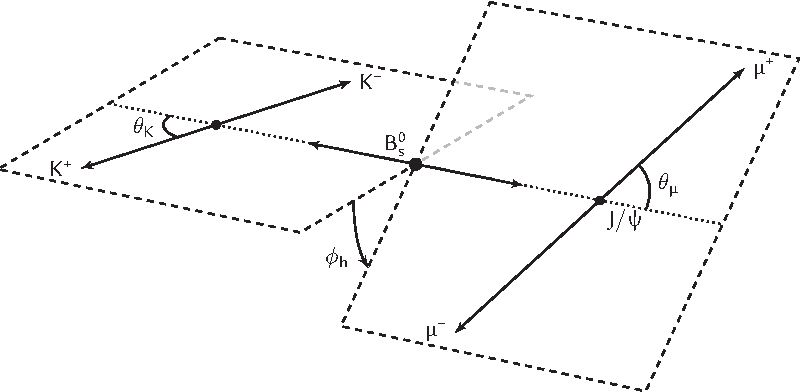
\includegraphics[width=\textwidth]{graphics/pheno/tikz/helAngles-crop}
  \caption{Definition of the decay angles in the helicity formalism.}
  \label{fig:helAngles}
\end{figure}

The change of variables from $\mpsiK^\text{2}$ and $\mKK^\text{2}$ to $\mKK$ and $\cthetaK$ introduces a Jacobian determinant in
Equation~\ref{eq:diffRateMsq}. Given that $\mKK^\text{2}$ does not depend on $\cthetaK$, when expressed in terms of the new variables, this
determinant reads $\frac{\partial\mKK^2}{\partial\mKK}\,\frac{\partial\mpsiK^2}{\partial\cthetaK}$. With the expression for $\mpsiK$,
\begin{equation}
  \mpsiK = \tfrac{1}{2}\,(\mBs^2 + \mJpsi^2 + 2\,\mK^2 - \mKK^2) + 2\,\frac{\mBs}{\mKK}\,|\pJpsi|\,|\pK|\,\cthetaK \ ,
\end{equation}
this is equal to $\text{4}\,\mBs\,|\pJpsi|\,|\pK|$, where $\mBs$ is the $\Bs$ mass, $\pJpsi$ the $\Jpsi$ three-momentum in the rest frame
of the $\Bs$, and $\pK$ the kaon three-momentum in the $\KK$ rest frame. Ignoring constant factors, the differential decay rate can now be
expressed as
\begin{equation}
  \label{eq:diffRateAngles}
  \ud\Gamma \propto |\pJpsi|\,|\pK|\, |\mathcal{A}(\Bstof)|^2\, \ud\mKK\, \ud\cthetaK\, \ud\cthetal\, \ud\phihel \ .
\end{equation}
The factors $|\pJpsi|$ and $|\pK|$ depend on the $\KK$ invariant mass, but not on the decay angles and can be absorbed in the
$\mKK$-dependent part of $|\mathcal{A}(\Bstof)|^2$ (see Section~\ref{sec:pheno_KKMass}).

The squared amplitude for the \BstoJpsiKK{} process can be obtained by working out expressions for $|\Af|^2$, $|\Abarf|^2$ and
$\Af^*\,\Abarf$ and combining these with the decay time dependence of Equation~\ref{eq:mixDecayDiffRate}. See Reference~\cite{Zhang:2012zk}
for an example of this approach for $\text{B}_q^\text{0}\to\Jpsihh$ processes in general.

However, it is often more convenient to order terms in the expression for the differential decay rate by intermediate resonant or
angular-momentum state rather than by decay-time dependence. Each term then has a distinct dependence on kinematic variables. For the
CP-violation analysis, a set of intermediate CP eigenstates is used to describe the decay.

The \BstoJpsiphi{} process is the decay of a spin-zero particle into two spin-one particles, which gives three intermediate
angular-momentum states. Describing the decay in terms of CP eigenstates, there is a state where the polarization vectors of the $\Jpsi$
and the $\phimesalt$ point along the helicity axis and two states where the vectors are transverse with respect to the helicity axis. The
former polarization is called \emph{longitudinal} and is indicated with ``0''. The two transverse polarizations are \emph{parallel}
($\parallel$) and \emph{perpendicular} ($\perp$), indicating the relative orientations of the two vectors in the transverse plane. The
\BstoJpsiKK{} S-wave gives a fourth intermediate state, indicated with ``S''. The longitudinal and parallel states are even under a CP
transformation, while the perpendicular and S-wave states are odd.

To derive an expression for the squared amplitude in terms of intermediate states it is necessary to go back to the expression for the
$\Bstof$ amplitude in Equation~\ref{eq:mixDecayAmps} and expand the decay amplitudes:
\begin{equation}
  \mathcal{A}(\Bstof) \propto g_+\, \Af + \qp\, g_-\, \Abarf = g_+\, \sum_i\Af[i] + \qp\, g_-\, \sum_j\Abarf[j]
  \ ,
\end{equation}
where $\Af[i]$ and $\Abarf[j]$ are the amplitudes for the $\Bsst$ and $\Bsbarst$ decays through intermediate states $i$ and $j$,
respectively. The dependence of the $\Bsst$ decay amplitude on final state kinematics is given by
\begin{equation}
  \Af[i] = \Ai\; \angAmp(\Omega)\; \mKKAmp(\mKK) \ ,
\end{equation}
where $\Ai$ is the complex-valued coefficient for amplitude $\Af[i]$, $\angAmp$ is the amplitude's dependence on decay angles
(denoted by $\Omega$), and $\mKKAmp$ is a model of the dependence on the $\KK$ invariant mass.

The $\Bsbarst$ decay proceeds through the same intermediate states as the $\Bsst$ decay and the respective amplitudes have the same
kinematic dependence. Therefore, the $\Bsbarst$ amplitude is obtained by replacing the coefficient $\Ai$ with $\Abari$. The total $\Bstof$
amplitude can now be expressed as
\begin{equation}
  \label{eq:amplitudeAmpLami}
  \mathcal{A}(\Bstof) \propto \sum_i \left( g_+ + \lamsi\, g_- \right) \Af[i] = \sum_i \timeAmp\,\Af[i]
  \ ,
\end{equation}
where $\timeAmp$\textequiv$g_+ + \lamsi\, g_-$ represents the decay-time dependence and the parameter $\lamsi$ is defined in
accordance with $\lamf$ (Equation~\ref{eq:mixDecayLamfDef}):
\begin{equation}
  \label{eq:amplitudeLamiDef}
  \lamsi\equiv\qp\frac{\Abari}{\Ai}
\end{equation}
The amplitude for the $\Bsbartof$ decay is obtained by interchanging $g_+$ and $g_-$ and multiplying by a factor $\pq$ (see
Equation~\ref{eq:mixDecayAmps}). Notice that this only affects the decay-time part of Equation~\ref{eq:amplitudeAmpLami}, i.e. the factor
$\timeAmp$.

For intermediate CP eigenstates, the parameter $\lamsi$ can be expressed as
\begin{equation}
  \label{eq:amplitudeLamiParam}
  \lamsi = \eta_i\,\lamsiAbs\,e^{-i\,\phisi} \ ,
\end{equation}
where $\eta_i$\texteq\tpm1 is the CP eigenvalue of the state, $\lamsiAbs$\texteq$\qpAbsAlt\big|\frac{\Abari}{\Ai}\big|$, and the
CP-violating phase $\phisi$ is given by $\phisi\text{\textequiv\tm}\arg\big(\frac{1}{\eta_i}\lamsi\big)$. If CP symmetry is violated by
the same amount for all intermediate states, the combination $\frac{1}{\eta_i}\lamsi$ does not depend on the state and $\phisi\to\phis$.

Squaring the magnitude of $\mathcal{A}(\Bstof)$ gives an expression that contains the products of the terms in
Equation~\ref{eq:amplitudeAmpLami} of the form $\Ai^*\Ai[j]\,\timeAmp^*\timeAmp[j]\, \angAmp^*\angAmp[j]\, \mKKAmp^*\mKKAmp[j]$.
Combining the interference terms with indices $ij$ and $ji$ gives
\begin{equation}
  \label{eq:sqAmp}
  |\mathcal{A}(\Bstof)|^2
    \propto \sum_i |\Ai\,\timeAmp\,\angAmp\,\mKKAmp|^2
      + \sum_{i\neq j} \Re( \Ai^*\Ai[j]\,\timeAmp^*\timeAmp[j]\, \angAmp^*\angAmp[j]\, \mKKAmp^*\mKKAmp[j] )
\end{equation}
The dependence on decay time, decay angles, and invariant $\KK$ mass of this expression are discussed in the following sections.
